\documentclass[12pt,a4paper]{article}

\usepackage[english]{babel}
\usepackage{amsmath}
\usepackage{upgreek}
\usepackage{paralist}
\usepackage{verbatim}
\usepackage{xfrac}

% types
\newcommand{\core}{\texttt{core} }
\newcommand{\kernel}{\texttt{kernel} }
\newcommand{\transition}{\texttt{transition} }
\newcommand{\seal}{\texttt{seal} }



% a core C
\newcommand{\C}{\mathcal{C}}
\newcommand{\V}{\mathcal{V}}
\newcommand{\G}{\mathcal{G}}
% OSTblock
\newcommand{\B}{\mathcal{B}}
\newcommand{\BS}{\operatorname{BS}}
\newcommand{\BE}{\operatorname{BE}}
% State root
\newcommand{\SR}{\operatorname{SR}}
% Storage root
\newcommand{\SO}{\operatorname{SO}}
% OSTblock gas limit
\newcommand{\OL}{\operatorname{OL}}


% make in the latest NIPS format (as of this writing, 2017)

\usepackage[nonatbib,final]{nips_2017}
%\usepackage[nonatbib,final]{nips_2017}

\usepackage{color}
\usepackage{graphicx}
\DeclareGraphicsExtensions{.pdf,.eps,.png,.jpg}		% search for .pdf, then .eps, then .pngs, then .jpg

% look in these subdirectories for graphics referenced by \includegraphics
% each entry must end with a /
\graphicspath{{figs/}{figures/}{images/}{./}}

\newcommand*{\red}[1]{ \color{red} #1}

%\usepackage{tabularx}
\usepackage{url}
\usepackage{amsmath}

% this is for environments \subfigure and \subtable
\usepackage{subcaption}

% These packages are FORBIDDEN
%%%%%%%%%%%%%%%%%%%%%%%%%%%%%%%%%%%%%%%%%%%%%%%%%%%%%%%%
%\usepackage{lmodern} % messes up \textsc
%\usepackage{cite} % messes up NIPS
%\usepackage{fullpage} % messes up NIPS
%\usepackage{natbib} % messes up NIPS
%%%%%%%%%%%%%%%%%%%%%%%%%%%%%%%%%%%%%%%%%%%%%%%%%%%%%%%%

\usepackage{array}			% replacement for eqnarray.  Must be BEFORE \usepackage{arydshln}
\usepackage{units}			% for \nicefrac{\alpha}{\beta}


\usepackage{amsthm}		% for theorems
\newtheorem{definition}{Definition}

% text looks a little better
\usepackage{microtype}

\usepackage{wasysym}

\usepackage{textcomp, marvosym} % pretty symbols
\usepackage{booktabs} 	% for much better looking tables

% for indicator functions
\usepackage{dsfont}

% For automatic capitalizaton of section names, etc.
\usepackage{titlesec,titlecaps}


\Addlcwords{is with of the and in}
\Addlcwords{of the}
\Addlcwords{and}
\titleformat{\section}[block]{}{\normalfont\Large\bfseries\thesection.\;}{0pt}{\formatsectiontitle}
\newcommand{\formatsectiontitle}[1]{\normalfont\Large\bfseries\titlecap{#1}}

\titleformat{\subsection}[block]{}{\normalfont\large\bfseries\thesubsection.\;}{0pt}{\formatsubsectiontitle}
\newcommand{\formatsubsectiontitle}[1]{\normalfont\large\bfseries\titlecap{#1}}





% for pretty Euler script
% \usepackage[mathscr]{euscript}
% \usepackage{bold-extra}





%\usepackage{subfig}
\usepackage{float} % for \subfloat

%%%%%%%%%%%%%%%%%%%%%%%%%%%%%%%%%%%%%%%%%%
%% More customizable Lists
%%%%%%%%%%%%%%%%%%%%%%%%%%%%%%%%%%%%%%%%%%
% Better symbols custom enumerative lists, define any symbol you'd like
% \usepackage{enumitem}


%%%%%%%%%%%%%%%%%%%%%%%%%%%%%%%%%%%%%%%%%%
%% Custom Symbols 
%%%%%%%%%%%%%%%%%%%%%%%%%%%%%%%%%%%%%%%%%%
% \xspace at the end of custom macros never screws up spacing.
\usepackage{xspace}



%%%%%%%%%%%%%%%%%%%%%%%%%%%%%%%%%%%%%%%%
%% Abbreviations you'll always want
%%%%%%%%%%%%%%%%%%%%%%%%%%%%%%%%%%%%%%%%
\newcommand*{\TODO}[1]{{\centering {\small \sffamily \color{red} #1} \vskip10pt }}
\newcommand*{\todo}[1]{{\small \sffamily [{\color{red} #1}]}}
\newcommand*{\q}[1]{{\small \sffamily [{\color{blue} #1}]}}
\newcommand*{\fix}[1]{{\sffamily [{\textnormal{\color{red} #1}}]}}



%-----------------------------------------------------------------------------
%  Cross references
%-----------------------------------------------------------------------------
% The following code defines how you make references to figures, tables, etc...
% It is defined in one place only, and can be modified for all references
% in the document at the same time.
% Instead of typing each time: "see Fig. \ref{myfig}" you can create a command
% \figref which will do the job. Then in text you only type \figref{myfig} and LaTeX
% will do the rest.
\newcommand{\tblref}[1]{Table~\ref{#1}}
%\renewcommand*{\figref}[1]{Fig.~\ref{#1}}
\renewcommand{\eqref}[1]{eq.~(\ref{#1})}
\newcommand{\Subref}[1]{(\subref{#1})}


\newcommand{\figref}[1]{Figure~\ref{#1}}
\newcommand{\Figref}[1]{Figure~\ref{#1}}
\newtheorem{theorem}{Theorem}
\newtheorem{lemma}[theorem]{Lemma}

%%%%%%%%%%%%%%%%%%%%%%%%%%%%%%%%%%%%%%%%

% for \sout{} for strikeout
% \usepackage[normalem]{ulem}


% for better manipulation of tables
\usepackage{makecell}
\renewcommand\theadfont{\bfseries}


%-----------------------------------------------------------------------------
%  Misc symbols that I like
%-----------------------------------------------------------------------------
\newcommand*{\opname}[1]{\operatorname{#1}}


\renewcommand*{\to}{\rightarrow}


%%%%
\graphicspath{{images/}}

\title{Mosaic\\\sc\Large{Running Meta-Blockchains to \\ Scale Decentralized Applications}}
\author{\textbf{B. Bollen, P. Gevorgyan, S. Khedar,}\\ \textbf{D. Kumar Nath, M. Schenck}\\ for OpenST Foundation \\ incomplete working draft}
\date{OpenST Mosaic v0.10 - September 2018}

\begin{document}

\maketitle

% TODO check bibliography
\begin{abstract}
This is a working draft summary of notes and whiteboard sessions as we have been iterating towards the implementation for Mosaic v0.10.
This is not the version intended for publication, and you are invited to review critically all content.
The code is work in progress at \verb|github.com/openstfoundation/mosaic-contracts|.
\end{abstract}

%
% Section
%
\section{Introduction}

%A blockchain derives correctness from full replication. Full replication is at the same time the strongest limitation to scaling a blockchain. Current proof-of-work, while secure has a transaction throughput that is constant with the number of (mining) nodes on the network. In order for blockchain networks to scale to billions of users, the network must at least scale (sub-)linear with the number of nodes contributing to the network.
%
%Three ingredients: divide the work up into shards, communicate between shards, and provide economic finality on each shard.
%
%These ingredients can be applied to layer1 blockchains, and then obtain blueprints like DFinity, Ethereum2.0. %TODO: which ones should we discuss in introduction? TON?
%
%The desired outcome of dividing the verification work into shards across nodes, is to parallelise the work load across nodes. When parallelising computations an orchestration % TODO: is "orchestration" the right word?
% strategy is required to avoid race conditions. One model to structure parallelised computation is by enforcing a strict ownership model on data and only a single thread can own and write to the data.
% 
% A blockchain naturally has a natural ownership model in the form of tokens. In Bitcoin unspent transaction outputs (UTXO) are an inherent ownership structure. In Ethereum's account model, any account can call on any other account, and there is not a direct ownership model. However, decentralized applications are often built around a token contract or use Ether to design the crypto-economic rules to interact with the decentralized application. Furthermore, non-fungible tokens create an ownership model for stateful data objects. % shit paragraph, but something
% 
% So at layer2 as tokens form the access-right to interact with a decentralized application, by the token-ownership model can be used to parallelise the execution of the decentralized application.
% 
% We define a \emph{shardable} application as a decentralized application that allows modification of its state based on ownership of tokens, or embeds state it computes on into non-fungible tokens. %rewrite
% \begin{align*}
%  A(t; x) \rightarrow A'
% \end{align*}
%
%-----

% Mosaic is parallelisation schema for decentralized applications.
Mosaic is a parallelisation schema for decentralized applications.
Mosaic introduces a set of Byzantine fault-tolerant (BFT) consensus rules to compose heterogeneous blockchain systems into one another.
Decentralized applications can use Mosaic to compute over a composed network of multiple blockchain systems in parallel.

A decentralized application is an application for which the computation is requested, performed, and paid for by independent actors.
To ensure correct execution of decentralized computations first an order on the inputs of execution must be determinable.
To date Ethereum is the leading network
% {TODO: quantify and reference; also define Ethereum as an instruction set, a mainnet network}
of nodes that enables developers to write and deploy code which can be called by independent users to collectively construct a shared state of the application.

% Ethereum is leading network of nodes for decentralized execution.
The Ethereum network achieves agreement on the collective state by constructing a blockchain.
A blockchain derives correctness from full replication of the computation by nodes and for Ethereum today the chain is appended through Proof-of-Work consensus.
%{TODO: give short intro, start from satoshi}
Proof-of-Work (PoW) introduces a block reward incentive for nodes to keep producing blocks and thereby securing the chain of historical blocks.
However, PoW produces a serial execution model and nodes cannot be collectively rewarded for the computation they all have to perform, which renders the system computationally inefficient\cite{verifiersdilemma}.

% NOTE: Ethereumv2 still needs to serialise all execution; DFinity starts from scratch 
Active research and implementation work is ongoing to scale Ethereum's transaction throughput by dividing the verification work into multiple sections, also referred to as \emph{shards}.
At the same time Ethereum is committed to moving from the probabilistic Proof-of-Work consensus engine to a BFT based Proof-of-Stake (PoS) consensus engine.\footnote{
	\url{https://github.com/ethereum/eth2.0-specs/blob/master/specs/casper_sharding_v2.1.md}
}
The outset of a BFT consensus engine is to collectively produce a blockchain which provably -- under certain honesty assumptions -- cannot finalise conflicting blocks.

% A second body of work constructs Proof-of-Stake blockchain systems by emulating Proof-of-Work's block proposal mechanism through pseudorandomly assigning to stakeholders the right to append new blocks\footnote{Peercoin, }.

% Bitcoin's arrival in 2009 is widely accepted as a turning-point, proving by demonstration, that a network can be constructed that balances economic interests of independent actors to collectively secure digital assets against double-spending. Ethereum innovates on Bitcoin by introducing a generalised scripting language, enabling a broad developer community for decentralized applications to grow.

Thus far a vision for a decentralized web has been a major driver of innovation.
However, to power global networks of billions of users and decentralized computation on vast decentralized data stores, it is reasonable to assume no single blockchain network will suffice as a backbone for all types of applications.
Much like the internet is a composed network of networks, we can conceive decentralized applications to transcend any single blockchain and execute across a network of blockchain networks.

In this work we detail two protocols.
The first, a layer-2 protocol, constructs \emph{meta-blockchains} on top of existing blockchain networks to extend their state space and transaction throughput capacity.
The second protocol, called a \emph{gateway}, acts as a message bus to send typed messages atomically between the underlying layer-1 blockchain and the meta-blockchain running on top of it.

Together these two building blocks can be used by decentralized applications to construct a parallelisation schema to increase %on-chain
computational capacity at lower transaction cost.
In its simplest form, a decentralized application can offload transaction processing to a single meta-blockchain.
More advanced applications can deploy logic across many meta-blockchains and process transactions in parallel while they can send asynchronous messages across meta-blockchains.

%%%%%%%%%%%%%%%%%%%%
% describe sections
%%%%%%%%%%%%%%%%%%%%


\section{Composing auxiliary systems into an origin}

A meta-blockchain composes transactions executed on an auxiliary blockchain system into an origin blockchain, such that the capacity of the origin blockchain extends and the auxiliary blockchain inherits the security properties of the origin blockchain.

To this end consider two blockchain systems, an origin blockchain $O$ with state transition rules $t_O$ which progress the state $\Sigma_O$ 
\begin{align} \label{state_transition_rules}
  t_O : \Sigma_O \rightarrow \Sigma_O'
\end{align}
and similarly consider an auxiliary system $A$ with state transition rules $t_A$ such that $t_A : \Sigma_A \rightarrow \Sigma_A'$.


Transition rules for the origin and auxiliary system can be similar but do not have to be.
In our discussion, when we need an example, we will reference to the origin blockchain as Ethereum (Byzantium), running Proof-of-Work, and for the auxiliary system we consider Go-Ethereum, running ``clique'' Proof-of-Authority (PoA).
We deliberately use PoA for our considerations for the auxiliary system to emphasise that the security for the composed auxiliary system is not derived from the consensus engine of the auxiliary system.
Rather the security properties of the composed system must rely only on the security properties of the consensus rules of the origin blockchain and on the Mosaic BFT consensus rules composing the auxiliary system into the origin system.\footnote{
	The block proposers of the auxiliary system do have the ability to censor transactions from the auxiliary system if they have an ability to collude.
}


On the origin blockchain we define a meta-blockchain $\mathcal{B}$ with a staked validator set $\mathcal{V}_\mathcal{B}$. The blocks $B_i$ of $\mathcal{B}$ are committed to a \emph{core} contract on origin $O$.
For a given history of $O$,\footnote{
	The origin blockchain $O$ might be probabilistically finalised, in which case a transaction to a contract can always assert that it is valid only on the intended branch of history by referencing a historical blockhash.
}
the meta-blockchain cannot fork if we enforce that block $B_{n+1}$ can only be (proposed and) committed after block $B_n$ has been committed.

% metablockchain
We define a meta-block $B_i(K, T, S): \Sigma_A \rightarrow \Sigma_A'$ to progress the state of the auxiliary system $A$, where we call $K$ the \emph{kernel}, $T$ the \emph{transition object} and $S$ the \emph{seal}.
A block $B_i$ at height $i$ of the meta-blockchain is committed with a seal $S$ when a $\texttt{+}\sfrac{2}{3}$ supermajority of the weighted votes has been verified.\footnote{
	While a vote counted on a BFT system itself is already BFT for a simple majority, %TODO : reference
	we still require a supermajority, because the votes to commit a meta-block will be collected on the auxiliary system for which there is no assumption it is BFT, and we want Mosaic to be able to finalise transactions on the auxiliary system before they are committed to origin.
}
We will detail later how the meta-block is constructed, but first we will describe the vote messages which, combined, seal a meta-block.

\subsection{Checkpoint finalisation - Casper FFG}
The reader is assumed at this point to be familiar with the work presented in \textit{Casper the Friendly Finality Gadget}\cite{casperffg} (FFG), as we will build on the logic and proofs presented there.
We will intend to align with definitions and notations where possible and highlight deviations where appropriate.
This section briefly (and incompletely) summarises core concepts from the paper, so that the shared concepts are established for the reader.

Casper FFG presents an algorithm to build up an overlay network of vote messages presented to a smart contract about the blocks already produced by the underlying network of nodes running the blockchain.
The overlay network aims to repeatedly economically finalise a single branch of the underlying network.
It does so by allowing staked validators to cast votes which together can construct a \emph{justified chain}.

A justified chain is formed by a sequence of \emph{supermajority links}, where a link identifies a \emph{source} blockhash $s$ and its height $h_s$ and a \emph{target} blockhash $t$ and its height $h_t$.
A vote message in Casper FFG is a link $\langle s, t, h_s, h_t\rangle_v$ signed by a validator $v$.
A $\texttt{+}\sfrac{2}{3}$ supermajority signing of the same link makes it a supermajority link which justifies the target block if the source block is itself already justified.\footnote{
	The genesis block of the auxiliary blockchain is considered justified by definition.
}

In the work it is shown that checkpoints along a justified chain can additionally be considered \emph{finalised}, if and only if they are justified themselves and their direct child checkpoint is justified.
It is then shown that, should validators finalise a checkpoint on a contradicting branch of the history of the underlying blockchain, minimally $\sfrac{1}{3}$ of the validator weight must have signed vote messages that violate either one of two rules: \emph{the Casper slashing conditions}.

These slashing conditions can be intrinsically validated given two signed vote messages from a validator $v$.
As such a validator must never sign two vote messages $\langle s_1, t_1, h_{s_1}, h_{t_1}\rangle_v$ and $\langle s_2, t_2, h_{s_2}, h_{t_2}\rangle_v$ for which either $h_{t_1} = h_{t_2}$ or $h_{s_1} < h_{s_2} < h_{t_2} < h_{t_1}$ holds.

It is additionally shown that validators can always finalise a new checkpoint, without being required to violate the slashing conditions, given that the block proposers propose blocks to append to the finalised fork, i.e. follow the fork selection rule of the overlay network.

\subsection{Finalising auxiliary systems}
Given a validator set $\mathcal{V}_\mathcal{B}$ staked for the meta-blockchain on origin, validators $v$ can submit, on the auxiliary system, vote messages about the auxiliary system of the form
\begin{align}\label{externalisedvote}
  \langle \tilde{T}, s, t, h_s, h_t \rangle_v
\end{align}
where $\tilde{T}$ is the keccak256 hash of the transition object $T$.

We introduce a transition object hash in the vote message to externalise otherwise intrinsic properties of the auxiliary system.
This transition object allows the Mosaic validators to coarse-grain and abstract the auxiliary system into a meta-blockchain when proposing meta-blocks on origin.

We require that any transition object is calculable by a smart contract on the blockchain in question for any finalised checkpoint along a justified chain.
For a given link, we define the transition object to refer to the state of the blockchain at source block $s$. % there could be multiple blocks at height h_s.
It then follows that for a given source blockhash $s$, $\tilde{T}$ is uniquely determined by $s$ and the same properties of accountable safety and plausible liveliness hold for a finalised checkpoint on a justified chain constructed by such \emph{externalised vote messages} (\ref{externalisedvote}), if we extend the slashing conditions to accommodate for the transition object hash.

A validator $v \in \mathcal{V}_\mathcal{B}$ must never sign two externalised vote messages $\langle \tilde{T}_1, s_1, t_1, h_{s_1}, h_{t_1}\rangle_v$ and $\langle \tilde{T}_2, s_2, t_2, h_{s_2}, h_{t_2}\rangle_v$ such that any of the following three conditions holds:
\begin{enumerate}
  \item $h_{t_1} = h_{t_2}$,
  \item $h_{s_1} < h_{s_2} < h_{t_2} < h_{t_1}$,
  \item $s_1 = s_2 \land T_1 \neq T_2$.
\end{enumerate}

As the slashing conditions can be intrinsically asserted to have been violated given two externalised vote messages by the same validator, there is no communication overhead to assert a possible violation of these conditions on the origin blockchain; even if the justified chain is being constructed on the auxiliary system.
As a result the validators in $\mathcal{V}_\mathcal{B}$ can be held accountable on the origin blockchain for their voting actions on the auxiliary system.
The slashing condition can be asserted on both systems and there is a clear incentive for the honest validators to assert any violation without delay on both the origin and auxiliary system, naturally synchronising the validator weights when such an event occurs.

We will later in this work address a dynamic validator set $\mathcal{V}_\mathcal{B}$, where validators can join and log out on the origin system.
However, already with a static validator set, we can observe that the finality gadget first introduced for (re)defining economic finality in layer-2 of Ethereum's PoW -- turning miners into mere block proposers and introducing a PoS (partial) consensus engine in the smart contract layer -- can also be applied to finalise an independent (auxiliary) system with a validator set whose stake is held on an external (origin) blockchain.

% TODO: EXPAND into a full section later
%\subsection{Expansion somewhere}
%Our final goal here is clear to see: by defining assets first on the origin blockchain before moving them onto the auxiliary blockchain economic finality as agreed upon by the validators staked on the origin blockchain is decisive. The nodes participating in the layer-1 auxiliary blockchain are forcefully turned into block proposers if their rewards are also awarded in assets held by the origin blockchain. By externalising all stake and all value of all assets, the auxiliary system is economically bound to follow the fork selection rule of the Mosaic validators.

\subsection{Observing origin}
\label{observing_origin}

Per construction the finalisation of the auxiliary system by the Mosaic validators economically binds the block proposers of the auxiliary system to the Mosaic fork selection.
By finalising the auxiliary system the Mosaic validators reach consensus about the auxiliary system itself.
However, to construct a meta-blockchain we will additionally require the Mosaic validators to reach consensus about their observation of the origin blockchain on the auxiliary system.
This is required so that message can pass bidirectionally between the chains.

To achieve it, the Mosaic validators construct a justified chain and finalise checkpoints along it for reported blocks of the origin blockchain on the auxiliary system.
The incentive structure is now reversed and the origin blockchain is in no way incentivised (nor should it be) to follow the fork selection rule of how a meta-blockchain's validator set finalised its observation of the origin blockchain.

In case the origin blockchain is probabilistically finalised, then it is always possible that the Mosaic validators of a given meta-blockchain running on top of the origin blockchain would economically finalise an observation of origin on the auxiliary system which is (later) reverted by the origin blockchain - even if they sufficiently trailed the head of origin.
Note that the validators cannot revert their finalised observation, because they would be required to sign vote messages which would violate the slashing conditions.

Under this scenario we must force the meta-blockchain to halt at the highest finalised checkpoint of the auxiliary system which was still consistent with its observation of the (now reverted) history of the origin blockchain.
This property can be enforced by including in the transition object of a justified chain of the auxiliary system $T^A$ information about the finalisation of the observation of the origin blockchain $T^O$,
\begin{align*}
  T^A_i = (O^j_f, \dots),
\end{align*}
where $O^j_f = f(T^O)$ is the function that returns the highest finalised block number $j$ and blockhash of the origin system as observed by the Mosaic validators for this meta-blockchain.

The origin blockchain can inspect $T^A$ to assert that the highest finalised observation of itself on the auxiliary system is within its current history.
Should this not be the case, then the origin blockchain must reject meta-blocks containing contradictory observations.

However, origin cannot directly assert that prior to the last finalised observation, there was no checkpoint finalised from a contradictory branch of its history, as the nodes on origin should not fully verify the transactions executed on the auxiliary system.
This is resolved by introducing an option to challenge a proposed finalised observation.

Assume an observed checkpoint $a$ was finalised on a contradictory branch of origin relative to the last finalised observed checkpoint $b$ included in $T^A$.
Any honest node can challenge the finalisation of $b$ on origin by presenting the finalisation of $a$ and demonstrating that $a \notin \text{history}(b)$.
Note that if validators would want to alter the finalised observation from $o \rightarrow a \rightarrow b$ to $o \rightarrow b$ they would have to produce vote messages violating the slashing conditions given the already existing vote messages.

Upon success the challenger is rewarded from the stake of the offending validators and the core contract must declare the meta-blockchain halted.

\subsection{Calculating the transition objects}

We construct a transition object $T^A$ to coarse-grain a vast amount of transactions processed on the auxiliary system under the state transition rules $t_A$ into a single, abstracted state transition that can be validated by the core contract on the origin blockchain (under the state transition rules of the origin blockchain $t_O$, eq. \ref{state_transition_rules}).

On the auxiliary chain with every block running parameters are tracked and these consist of the latest finalised observation of the origin blockchain $O^j_f= f(T^O)$, the \emph{accumulated transaction root} $r_i$, the \emph{accumulated gas} $g_i$ consumed, and the current \emph{dynasty number} $d$ on auxiliary.
The transition object $T^A$, however, is updated at every justified checkpoint $s$ with height $h_s$ and we write for a given meta-block height $n$:
\begin{align*}
  T^A_{n,d}(s) = (d, O^{j_d}_f, r_d, g_d, \tilde{K}_n)
\end{align*}
where $\tilde{K}_n$ is the keccak256 hash of the kernel $K_n$.

A smart contract calculates the parameters that go into $T^A$ for every block.
Therefore, the validators have to report the block header of every block to the smart contract.
If the reported block is within the most recent 256 blocks of the auxiliary blockchain,\footnote{
	This is specific to the Ethereum virtual machine, but the logic can be applied for other blockchain systems as well.
}
then the smart contract can verify its correctness by accessing the corresponding block hash.
If the validators fall behind more than 256 blocks in reporting, they can report more than one block per new block in order to catch up.
The smart contract will record all reports, but only mark them as valid if they build a chain that reconnects to a block hash within the most recent 256 blocks of the current branch.

Tracking of $T^A$ begins at the genesis checkpoint.
For the genesis checkpoint, the accumulated transaction root is defined as the transaction root of the block, the accumulated gas consumed equals the gas consumed in the block, and the current dynasty number is 0.
For all subsequent blocks, the accumulated transaction root $r_i$ at block height $i$ is $\text{keccak256}(r_{i-1}, R_i)$, where $R_i$ is the transaction root of the block at height $i$.
The accumulated gas consumed $g_i$ at block height $i$ is $g_{i-1} + G_i$, where $G_i$ is the gas consumed in the block at height $i$.
The dynasty number equals the number of finalised checkpoints in the chain from the root checkpoint to the parent block, carrying over the definition of dynasty number as in Casper FFG \cite{casperffg}.

Further, we introduce a constant \emph{core identifier}, a 256-bit string where the first 12 bytes are a constant specifying the origin blockchain and the rightmost 20 bytes are determined by the smart contract address of the core contract on the origin blockchain.
Rather than storing the core identifier in the transaction object, it can be included as a constant in the signing string for vote messages to ensure vote messages are valid only about the intended meta-blockchain.

% Note to self: follow up on the thinking that by externalising the transition object into the vote message allows the calculation to be done in the node, not in the contract.

\begin{figure}
    \centering
	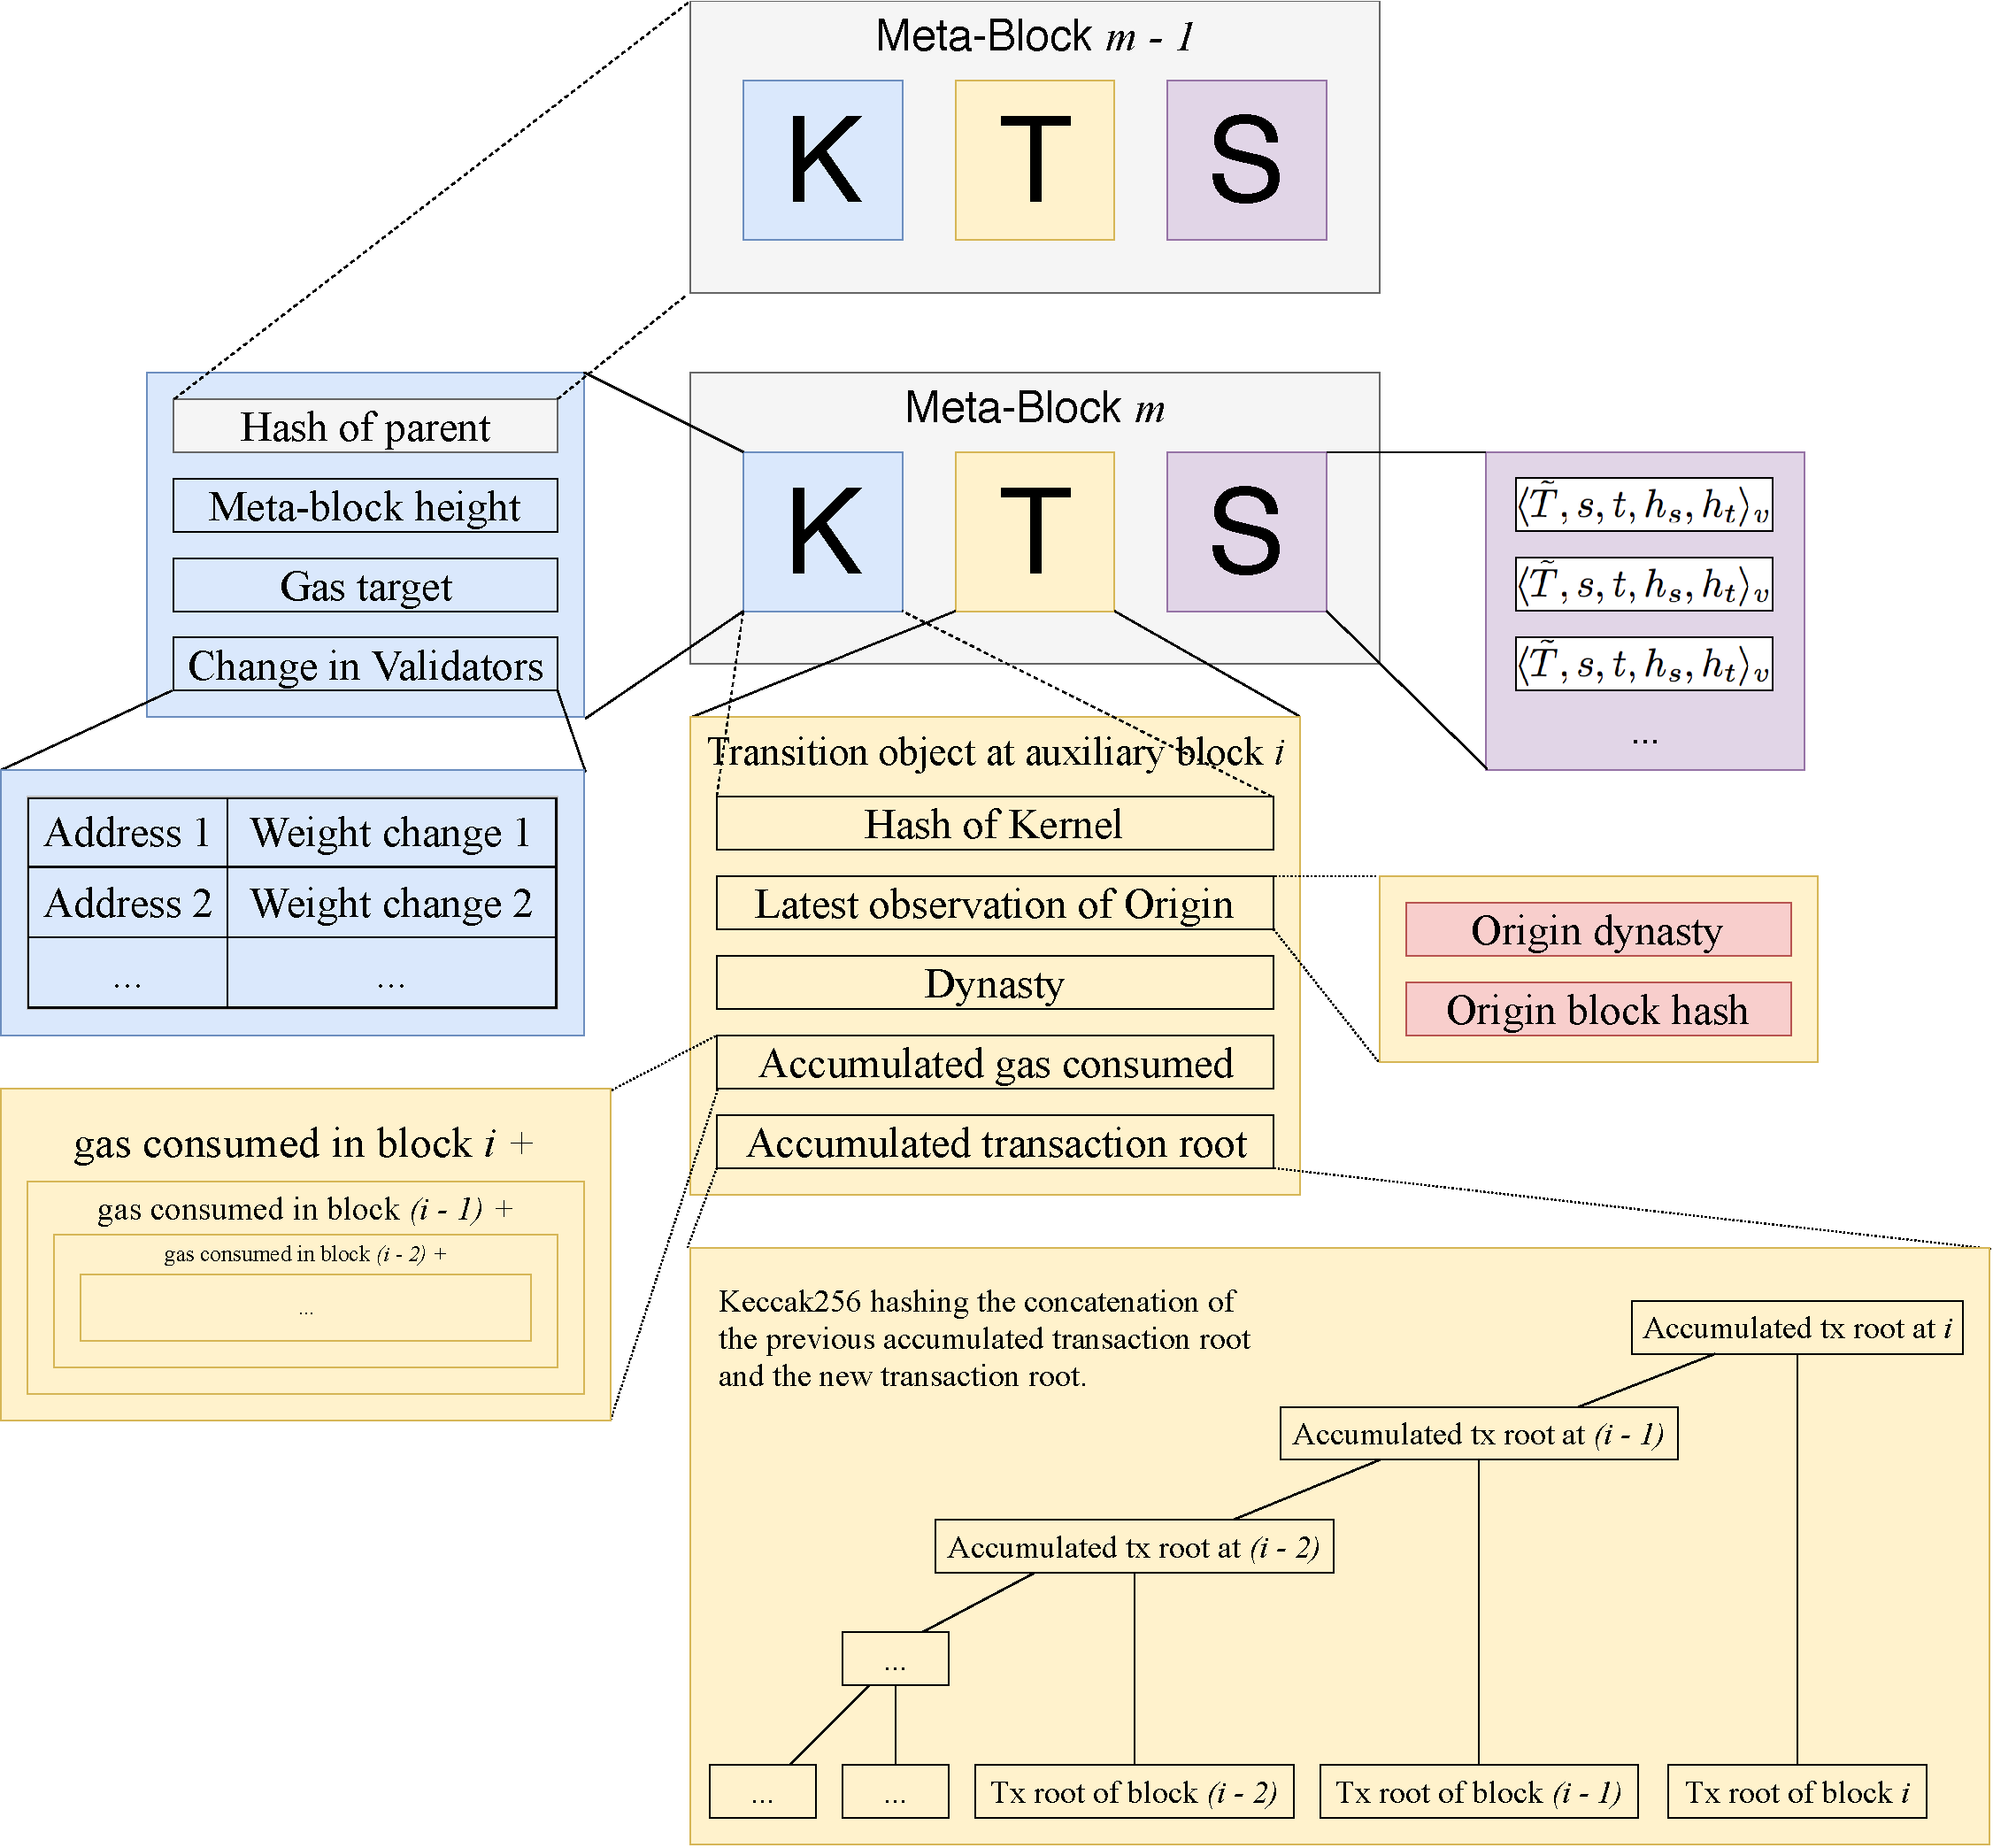
\includegraphics[width=\textwidth]{meta_block}
	\caption{\textbf{Anatomy of a meta-block.}
		The meta-block consists of a kernel, a transition object, and a seal.
	}
	\label{fig:meta_block}
\end{figure}

\subsection{Proposing meta-blocks on origin}

For a meta-blockchain $\mathcal{B}$ the chain can be appended by proposing and committing new meta-blocks $B_n(K_n, T^A_n, S_n)$ in the core contract on the origin block\-chain.
The genesis meta-block $B_0$ is considered committed per definition.

The kernel $K_n$ is a tuple $(n, \tilde{p}_n, \Delta\mathcal{V}_{\mathcal{B}_n}, gp_n, gt_n)$ fully determined by and stored in the core contract on the origin blockchain. %The height $n$ strictly increases by one every time a meta-block is committed into the core contract.
On a given branch of the origin blockchain a meta-blockchain cannot fork.
The act of committing a meta-block $B_{n-1}(K_{n-1}, T^A_{n-1}, S_{n-1})$ activates the new kernel $K_n$ at height $n$ and \emph{opens} the core contract to accept proposals of the form $B_n(K_n, \cdot, \cdot)$.
The kernel further specifies the \emph{parent hash} $\tilde{p}_n$, the \emph{updated validator weights} $\Delta\mathcal{V}_{\mathcal{B}_n}$ to declare new validators joining and existing validators logging out. The kernel includes a voted-upon \emph{gas price} $gp_n$ for the gas that will be consumed in the upcoming meta-block $B_n$ as rewarded to the Mosaic validators.\footnote{
  A meta-blockchain has a double gas market.
  First the known gas market exists where users set a gas price in the transaction that gets executed on the auxiliary blockchain and the gas rewards go to the block proposers of the auxiliary system.
  A second, new gas market is created by requiring the block proposers to pre-deposit gas rewards for several meta-blocks in advance.
  Mosaic validators are rewarded upon committing a meta-block on the origin blockchain for the total gas consumed in that meta-blockchain at the agreed-upon gas price $gp_n$ for that meta-block $B_n$.
  Details in later section.
}

\paragraph{gas target} Lastly $gt_n$ is the \emph{gas target} which introduces a forcing function on the total amount of gas that can be consumed in the meta-block $B_n$.
The earliest finalised checkpoint at which the gas target has been consumed by the meta-block must be committed to the origin blockchain by the validators.
We highlight that this is not a maximum gas limit, because it cannot be guaranteed that a checkpoint can be finalised before a hard gas limit would be surpassed. Rather validators would gradually lose part of their stake as a function of the number of finalised checkpoints they failed to commit after the gas target has been surpassed.

To show that validators can be held accountable, assume the finalised checkpoint $s_d$ has been committed which surpassed the gas target and has dynasty number $d$.
Now assume there exists a finalised checkpoint $s_{d'}$ which also has surpassed the gas target but has a lower dynasty number $d' < d$, but was not committed before $s_d$.
Any honest node can present the $s_{d'}$ and the core contract can assert the gas target had been consumed at a lower dynasty number than what is committed and reward the challenger.

\paragraph{committing a meta-block} Given a committed meta-block $B_{n-1}$ at height $n-1$ a proposal for a meta-block $B_{n}(K_{n}, T^A_{n}, \cdot)$ at height $n$ is a valid proposal if validity assertions for the transition object $T^A_n$ hold.  These validity assertions require that the dynasty number and the gas consumed are strictly increasing compared to the transition object committed $T^A_{n-1}$. The transition object $T^A_n$ must reference the correct kernel $\tilde{K_n}$. It must be checked that the latest finalised observation of origin is within the history of the current state. Furthermore  a brief challenge period exists where the transition object can be contested on the grounds that it contains a prior observation of origin that contradicts the current history of origin, as explained above in section (\ref{observing_origin}).

It now follows that for a given active kernel $K_n$ multiple proposals $T^{A}_{n,d}$ can be submitted to the core contract for different dynasty numbers $d$.  These proposals are no longer contradicting versions of the history, rather they are ordered, sequenced snapshots of possible state transitions $B_{n,d_{n}}(\Sigma_{A,d_{n-1}})$ that can be committed onto origin as a new meta-block.

To commit a meta-block then requires selecting among the valid proposals a dynasty number $d_n$ for which the meta-block will be closed. This selection occurs automatically by sequentially verifying the vote messages on the origin blockchain.
The meta-block $B_n(K_n, T^A_n, S_n)$ will be committed with the seal $S_n$ which first asserts a $\texttt{+}\sfrac{2}{3}$ supermajority of the voting weight $\mathcal{V}_{\mathcal{B}_n}$ for a valid proposal in the set of valid proposals
\begin{align*}
  \{S_{n,d}\} = \left\{\left\{\langle\tilde{T}^A_{n,d}, s, t, h_s, h_t\rangle_v\right\}\right\}
\end{align*}
where it is required that the supermajority link finalises the source $s$.
As such we require that $h_t - h_s = 1$ and the source $s$ must have been justified.

Following the same reasoning as presented in section (\ref{observing_origin}) we can assert whether or not the finalised checkpoint $s$ was obtained through an unbroken justified chain leading up to the finalised checkpoint, by allowing for a challenge\footnote{A challenger must always put forward a sufficient stake to underwrite the cost implied by her challenge.} to be raised against a proposed transition object $T^A$ included in a vote message $\langle\tilde{T}^A, s, t, h_s, h_t\rangle_v$.

However, recall that in the case of verifying observations of origin (\ref{observing_origin}), origin itself can act as an arbiter because origin can rely on its own history.
Our concern now is to assert that the state transition to $s$ from the last committed state $B_{n-1}$ is a valid state transition according to the state transition rules $t_A$ of the auxiliary system.

\paragraph{proof} Assume first a contradictory finalisation $s'$ of the auxiliary system relative to $s$ exists. This implies that more than $\sfrac{1}{3}$ of the validator weight can be slashed.
The core contract on origin must declare the meta-blockchain halted when it can slash more than the safety threshold of $\mathcal{V}_{\mathcal{B}_i}$ at a single meta-blockchain height $i$.\footnote{When a meta-blockchain has been halted, assets and stateful objects can be recovered on the origin blockchain at any later time with Merkle proofs against the last committed state root of the meta-blockchain.
We will detail the conditions under which a meta-blockchain must halt and how the recovery processes can work later in this writing.}

Alternatively no contradictory finalisation $s'$ of the auxiliary system relative to $s$ exists.
Under the security model assuming a $\texttt{+}\sfrac{2}{3}$ supermajority of the validator weight is honest, it follows that the proposed state transition to $s$ has been obtained through honest verification of all transactions under the state transition rules $t_A$.

Before continuing we summarise that the proposal mechanism to commit a meta-block is asynchronous, requires no leadership-selection and is proven to be Byzantine fault-tolerant under the security model of an honest supermajority.

\subsection{Beyond an honest supermajority}

While the origin blockchain protects assets from being double-spent, users in a meta-blockchain could see their funds stolen if more than a supermajority of the open validator set would collude to violate the transition rules $t_A$. 

We identify at least three active research topics which can allow to push the security model radically further in an efficient way; namely that (up to) a \emph{single} honest observer can hold all validators accountable when a proposal for committing a meta-block to the origin blockchain would violate the state transition rules $t_A$.
It is outside the scope of the current work to explore in-depth, but they are worth summarising below as future work paths.

\paragraph{observer network} In \textit{A Guide to 99\% Fault Tolerant Consensus}\cite{honestobserver} V. Buterin recaptures an existing algorithm by L. Lamport (1982) to describe how a \emph{latency-dependent} network of observers can be retrofitted on top of a \emph{threshold-dependent} consensus algorithm - in casu our here work as derived from Casper FFG - to introduce a \emph{strong-finality} upon the finalised history constructed by the Mosaic validators arbitrarily pushing up the fault-tolerance at the cost of requiring more observers and a longer time to eventually commit (a strongly finalised proposal).
%We leave as an open question whether the origin blockchain can facilitate the global timing of the \emph{always-online} network of observers.

\paragraph{truebit} A second worthwhile path is to apply the \textit{TrueBit}\cite{truebit} protocol to challenge a state transition $T^A$ proposed by a subset of the validators $\mathcal{V}_{\mathcal{B}_i}$.
The validators $\{v\}$ who have signed vote messages $\langle\tilde{T}^A, s, t, h_s, h_t\rangle_v$ can be seen as the (collective) \emph{solvers} of the off-(of-origin-)chain computation to transition the state $B_{n-1}$ to the proposed solution $s$ given the set of transactions specified by the accumulated transaction root $r_{h_s}$.
The computation at hand is the execution of the virtual machine that implements the state transition rules $t_A$.

If less than $\sfrac{1}{3}$ of the validator weight loses the verification game to a challenger, their stake can be taken as the reward for the challenger, on top of the shared interest of all participants in the meta-blockchain for only correct proposals to be committed to the origin chain - removing the need for a jackpot and a \emph{forced-error}.
The verification game can be seen as an extension to the slashing conditions strengthening the accountable safety of the meta-blockchain to hold a minority of the validators accountable for violating the state transition rules $t_A$.
This is made possible because the validator stake has been externalised on the origin blockchain with an independent (assumed correct) consensus mechanism.

If more than $\sfrac{2}{3}$ of the validator weight signed the vote message which was challenged and lost the verification game, their stake is the reward for the challenger, and the meta-blockchain must be declared halted by the core contract.

\paragraph{argument of knowledge} A third strategy can be constructed by requiring any of the challenged validators of a proposal $T^A$ to present an \emph{argument of knowledge}, eg. using \mbox{zkSNARKs} generated after being challenged, to cryptographically prove that the block $s$ has been obtained by correctly applying the state transition rules $t_A$ recursively on each parent block building up from the committed block found in $B_{n-1}$.

The costs both in time and expense to generate this proof by a validator scale at first approximation linearly with the gas consumed in the proposed meta-block $B_n$.
The transition object $T^A$ to commit this meta-block tracks the gas consumed, so the core contract can require that the challenger puts forward a sufficient stake to substantiate her claim.

% TODO: research state of art on hardware requirements
There are open considerations regarding the (economic) feasibility of requiring all validators to be able to generate such a proof on commodity hardware.
The task of generating these proofs could be designated to a specialised node, but an incentive problem arises when it is economically unattractive to run such a node considering it is unlikely that a proposal would be challenged.

We have gone beyond the assumption of an honest supermajority of validators by considering three strategies discussed in the field to radically improve the security model; up to the point where a single honest observer can cost-effectively challenge the validator set on the origin blockchain.

%We welcome other teams to explore and collaborate with their implementations and improvements to test these and more strategies to tighten the security model.

\subsection{Dynamic set of validators}

The set of validators for the meta-blockchain $\mathcal{B}$ must be dynamic to allow new validators to join and for validators to safely exit from their responsibilities. It is defined for each meta-block height $i$ and we note $\mathcal{V}_{\mathcal{B}_i}$.
 
The set of Mosaic validators needs to be able to change.
A validator can join the set of validators by sending a deposit transaction to the stakes contract on origin.
The amount of stake of the validator is based on the amount of value that the validator sends with the deposit transaction.
% TODO: should it say staking is done in OST, ERC-20, or just value?
% TODO: will the rewards go to the stake? will they also go to the weight?

When a validator wants to leave the set of validators, it sends a logout message to the stake contract on origin.
The validator's weight is reduced to zero, therefore the validator leaves the set of validators.
% TODO: is 4 months fixed or should it say something variable.

\begin{figure}[htb]
    \centering
	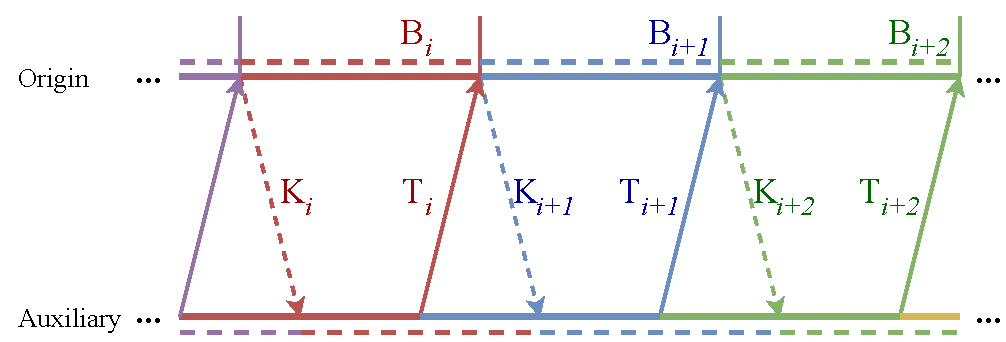
\includegraphics[width=\textwidth]{transition}
	\caption{\textbf{Transition.}
		After the transition object $T_i$ is committed on origin, the opening of the new kernel $K_{i+1}$ is confirmed on auxiliary.
		On auxiliary, meta-block $B_{i+1}$ retroactively opens from the point where $B_i$ closed.
		The set of validators, however, only changes at the time of confirmation.
		The dashed line under auxiliary shows the active set of validators.
	}
	\label{fig:transition}
\end{figure}

When a validator casts a vote on auxiliary, the vote carries a specific weight.
The initial weight of a new validator is equal to the stake on origin.
When we say that a vote receives a $\sfrac{2}{3}$ majority, we mean that at least $\sfrac{2}{3}$ of the total voting weight on auxiliary have cast that vote.
A validator's stake may be reduced to a non-zero value, e.g. by slashing.
However, in any slashing case the weight will always go to zero immediately.

We defend against long range revision attacks the same way casper does.
Four months after the validator left the set of validators, the validator can withdraw its stake.

Casper FFG\cite{casperffg} defines a stitching mechanism for a changing set of validators.
It prevents a case where a significant change in validators from one dynasty to the next could result in conflicting finalised checkpoints on different forks.
They define a forward validator set and a rear validator set based on the start dynasty and end dynasty of a validator.
In the case of Mosaic, however, validators do not join and leave the set of validators within two dynasties, but rather two meta-blocks.
When a validator sends a deposit or logout message at meta-block height $i$, the change is announced to auxiliary with the opening of meta-block $i+1$.
% TODO: any existing notation for meta-block height?
The auxiliary system will update the validator's weight with the opening of meta-block $i+2$ and the validator will join or leave the set of validators. We call that meta-block the start meta-block or end meta-block.
Following this change, the forward and rear validator sets are based on the start meta-block and end meta-block, respectively, instead of the start dynasty and the end dynasty.

 In the same way, an ordered pair of checkpoints $(s, t)$, where $t$ is in meta-block $B_i$, has a supermajority link if both at least $\sfrac{2}{3}$ of the forward validator set and the rear validator set of $B_i$, respectively, have published vote $\langle \tilde{T}, s, t, h_{s}, h_{t}\rangle_v$.

The same public key can only deposit and withdraw once.
It cannot join the set of validators multiple times or change its stake.

NOTE: weight = stake x reputation

When a meta-block has been committed on origin, the Kernel of the newly opening meta-block can be confirmed on auxiliary.
The state root of origin is regularly transferred to auxiliary and finalised.
By means of a Merkle proof against that known state root, the content of the Kernel can be made available to auxiliary.
Auxiliary will note the update of the validator weights for the meta-block height of the opened meta-block plus one.
The validator set changes on auxiliary at the time the kernel opening is confirmed.
Even though the kernel opening retroactively opens the meta-block on auxiliary from the first block after the last finalised checkpoint in the meta-block that precedes the opening one, the validator set only changes at the point of the confirmation.
When the Kernel at height $i$ is confirmed on auxiliary, the validator set $i+1$ becomes the active set of validators.
The validators that logged out on origin before the opening of $K_i$ will be in the rear validator set of $K_{i+1}$ and leave the validator set when $K_{i+2}$ is confirmed.

\begin{figure}[htb]
    \centering
	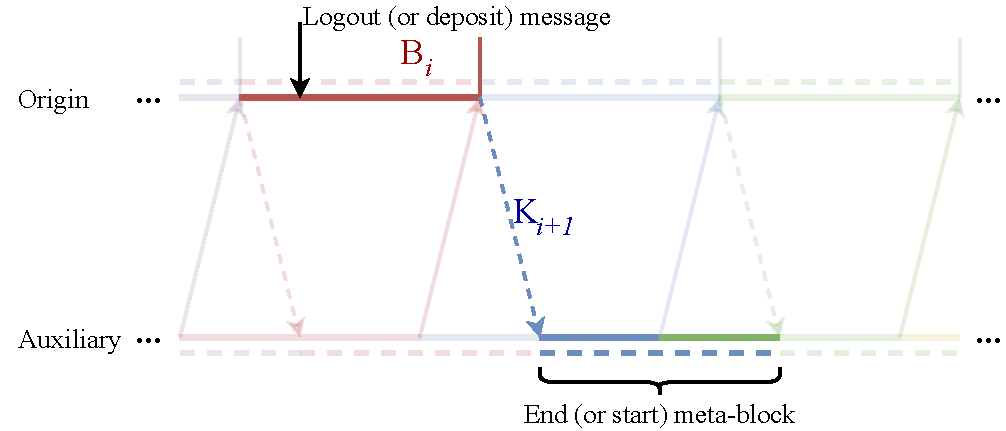
\includegraphics[width=\textwidth]{dynamic_validators}
	\caption{\textbf{Dynamic set of validators.}
		The validator sends a log out message (or a deposit message) in $B_i$.
		The change in the set of validators is transferred to auxiliary as part of kernel $K_{i+1}$ that gets confirmed.
		The validator does its last round in the rear validator set on auxiliary.
		The validator's weight drops to zero when $K_{i+2}$ is confirmed (or the validator joins in the forward set of validators).
	}
	\label{fig:dynamic_validators}
\end{figure}

%The logic is similar to that of Casper with the notable difference that, instead of dynasties, we use OSTblocks (described below).
%When a potential validator sends a \emph{deposit message} on origin at OSTblock height $\alpha$,
%then the validator will be announced as part of the next set of validators in the header of OSTblock $\alpha+1$ and 
%the validator $\upnu$ will join the validator set at OSTblock height $\alpha+2$.
%% TODO a lot copied from Casper. OK? Required?
%Analogous to Casper, we call $\alpha+2$ the validator's \emph{start OSTblock}, $\BS(\upnu)$.
%If a validator $\upnu$'s withdraw message is included on origin's blockchain during an open OSTblock $\B_\alpha$,
%it similarly leaves the set of validators at OSTblock height $\alpha+2$.
%We call $\alpha+2$ the validator $\upnu$'s \emph{end OSTblock} $\BE(\upnu)$.

%related work: cosmos and polkadot each introduce a cosmos hub or relay chain as a new 
% historic background of Ethereum driven to decentralise the world wide web framework; Mosaic is driven to decentralise high-performance computation
% Mosaic 


% design philosophy: heterogeneneous composition of systems; different applications have different optimal specifications/requirements;
% allows collective innovation


% related work: primea DFinity consensus-primea-VM concurrency in contracts; asynchronous message passing; partial ordering of messages (explicit in Mosaic; correct by construction); nonatomic by default...8-0; atomicity and reverts

% Mosaic: async message passing between meta-blockchains; synchronous message passing within one blockchain
%

% communication semantics

% locality of stateful data to compute on. move computation where the data already is; data in a shard is fully replicated

% payment channels, and state channels are logic-specific; plasma chains logical continuation of state channels; but different applications cannot send synchronous messages to each other across state channels or plasma chains. off-chain layer2 solutions; closing always leads to challenge period; meta-blockchain moves block proposal off-chain
% mosaic is an on-chain layer2 solution.
% comparison to state-channels:
% data-availability -> validator pool rewarded for keeping full copy of state; not required by end-users
% cost opening-closing channel: meta-blockchain is permanently open, applications and users can move in- and out of meta-blockchains; cost updating in meta-blockchain higher than state channel, but lower than on mainnet
% privacy: meta-blockchains are transparancy tool; lower cost for execution allows better substrate for homomorphic encryption, proxy-re-encryption and zk-proofs
% fast asynchronous finality
% counterfactual/L4 "build state-channels into their application"
% plasma: root contains "state-transition rules" <-> Mosaic Core does not have specific transition rules; split chain from 

\subsection{gas markets}

Users of the auxiliary system pay gas fees to the block proposers of the auxiliary system for every transaction.
Similarly, users of the origin blockchain pay gas fees for their transactions on origin.
Due to the limit on the number of transactions included in each block, the gas price is determined in a system of supply and demand.
When many users want to include many transactions in blocks, possibly above the limit, the average gas price will naturally rise and vice versa.

The meta-blockchain includes transactions from auxiliary.
Users of the auxiliary system already paid a gas fee for when the transactions were included in an auxiliary block and cannot be expected to pay another fee later on.
Still, it is desired that the validators have an incentive to commit meta-blocks on origin, as it is a pre-requisite for anyone to transfer value from auxiliary to origin.

Mosaic provides two incentives for the validators to do so:

\begin{enumerate}
	\item The validators receive a gas fee for a committed meta-block, based on the gas that auxiliary consumed for all auxiliary transactions that exist within that meta-block.
	\item The validators get rewarded on auxiliary. In order for them to move the rewards to origin, they must first commit a meta-block.
\end{enumerate}
% TODO: do we even need the gas fee or is "2." plus the gas target sufficient?

\paragraph{Gas fees.}
For every meta-block, validators get rewards based on the amount of gas that was consumed on auxiliary within that meta-block.

The amount paid out to a single validator address on auxiliary equals
\begin{align*}
  \frac{w_v}{w} \cdot g \cdot gp
\end{align*}
where $w_v$ is the weight of the validator, $w$ is the total weight of all validators, $g$ is the accumulated gas of the meta-block, and $gp$ is the agreed upon gas price.

However, this amount increases with increasing size of a meta-block.
% TODO: agree on gas price (who, when, where).

\paragraph{Validator rewards.}
Whenever someone commits a meta-block on origin, the meta-block closes, a new meta-block opens, and someone confirms the kernel of the newly opened meta-block on auxiliary.
The auxiliary system tracks the total gas consumption per checkpoint and can therefore calculate the amount of gas consumed in the closed meta-block on-chain.
The gas consumed of a meta-block is merely a mirror of the gas that all auxiliary transactions within that meta-block consumed on auxiliary.

A smart contract on auxiliary pays out a fee to the validators based on the gas consumed in the closed meta-block.
In order for the auxiliary smart contract to be able to do the pay-out, the block proposers of auxiliary must deposit sufficient value for multiple future meta-blocks in said contract.
Block proposers have an interest in confirmed meta-blocks on origin.
They earn on auxiliary for proposing blocks and they can only transfer their value to origin after a meta-block is committed.
Furthermore, an auxiliary system with more frequent meta-block commits could be more interesting to users and therefore produce more gas rewards for the block proposers.

If block proposers would fail to produce a sufficient deposit for validator rewards, validators would most likely switch to a more profitable auxiliary chain.

%
% Section
%
\section{A mosaic of cores}

summary:
by constructing asynchronous BFT consensus rules to compose a heterogeneous auxiliary blockchain into the origin blockchain, we leverage the security of the origin blockchain to asynchronously finalise the transactions on the auxiliary blockchain.
As there are no time constraints or time-outs in the Mosaic consensus rules, the limited processing capacity of the origin blockchain does not undercut the ability to compose many auxiliary systems into the same origin blockchain.
This enables Mosaic to run many meta-blockchains in parallel, additively improving the total transaction capacity, but keeping a bound on the cost imposed on the origin blockchain.
%% 
%A blockchain relies on each full node replicating all transactions to obtain and verify independently the correctness of the current state. Full replication at the same time impedes scalability.
%
%% extend state space of origin
%Mosaic sets out to leverage the security and liveliness properties of the origin blockchain. Mosaic allows to create a new state space and compose it into the origin state space so that it suffices to verify the origin state space and the extended state space the node is 
%
%Mosaic is a framework to increase the transaction throughput of an origin blockchain (e.g. Ethereum) by finalising transactions off of the origin blockchain. Finalised transactions can be committed asynchronously in bulk onto the origin blockchain. 

\begin{comment}
\section{the dry stuff}



\subsection{Origin}

the origin blockchain is the assumed BFT blockchain for upon which Mosaic cores are deployed to extend the origin state space.

\subsection{Mosaic consensus rules}

Build on Casper FFG.

Validator can sign a vote message 

\begin{align*}
  \langle T, s, t, h_s, h_t\rangle_v
\end{align*}

slashing conditions for a validator :
\begin{enumerate}
  \item $h_t \neq h_{t'}$
  \item inclusion not allowed $h_{s_1} < h_{s_2} < h(t_2) < h_(t_1)$
  \item $s_1 = s_2 \land  T_1 \neq T_2$
\end{enumerate}


\subsection{Stake}

Stake defines the validator list and their voting weight derived from their deposited stake.

\subsection{Core}

Core is a meta-blockchain defined on origin. On core a meta-block can be proposed and committed. A meta-blockchain cannot fork (assuming the origin blockchain has not forked).

\subsection{meta-block}

A meta-block defines a block transition for the core $c$

\begin{align*}
  B : S_c \rightarrow S_c'
\end{align*}

and a meta-block is composed out of three components. A meta-block has a \kernel $K$, a \transition $T$ and a \seal. The kernel is determined by the \core contract on the origin chain. The transition is generated in the finalisation process by the validators on the auxiliary chain. Lastly the seal is generated by the core contract on origin as the validators verify their vote messages. The meta-block's hash is derived from the kernel and the transition $(K, T)$.

The kernel $K$ has five fields. \texttt{height} counts the number of committed parent meta-blocks. The genesis meta-block has height zero. \texttt{parentHash} refers to the meta-block hash of its parent. The kernel further specifies the \texttt{gasPrice} the proposers are willing to pay the validators for committing the meta-block. Lastly the kernel contains an update-insert list of validators and their updated weights. Validators who's weight is set to zero are removed from the validator list.

\subsection{Block Store}

Block store is a representation of a blockchain on-chain. 

\subsection{Polling place}

Polling place tracks the weight of the validator set and collects vote messages about links between checkpoints.


\section{Gateway}

\subsection{MessageBus}

Message bus allows abstraction of logic to pass a message from bidrectionally between origin and auxiliary.
Declaration, confirmation and progression and optional reverting of messages.

\subsection{ERC20-typed}

\subsection{Kernel-typed}

\section{Running origin and auxiliary chains}
\label{subsec:mosaic}



%Quote FFG slashing conditions and voting rules.

% General assumption
%Each validator can verify the blocks $a_i$ it has received (incomplete view).
%Origin is byzantine fault tolerant -> each validator can assert (prob) finality of the state of origin.

% See lemma plus accountability must be done twice in two directions

% TH 1 and 2 Vo can be slashed for the actions of Va

% All theorems and lemmas assume liveliness of Origin
\end{comment}

\begin{comment}
We assume without loss of generality that for every validator-address $v^O$ in the validator set $\V^O$ on origin a corresponding,
unique validator-address $v^A$ on auxiliary $A$ can be associated and we call the resulting validator set $\V^A$,
the validator set on $A$. A single actor is assumed to control and be responsible for both $v^O$ and the associated $v^A$.
On origin $v^O$ will always be held accountable for any signed message by $v^A$ on $A$, because and only $v^O$ has stake on origin.


\begin{lemma}[Remote Accountability]
	\label{lemma:remoteaccountability}
	A vote on $A$ that violates a Casper Commandment can be punished on $O$.
	\begin{proof}
		% TODO @benjaminbollen removed the lemma so we can not reference it anymore
		Given lemma~\ref{lemma:mapping}, a violation of either Casper Commandment can be proven on $O$ without the respective transaction residing on $O$.
		If a validator $\upnu^A$ published two distinct votes for the same target height, the relevant votes can be presented on $O$ and the signature can be validated.
		An offending validator $\upnu^O$ can be identified according to lemma~\ref{lemma:mapping} and its deposit slashed.
		The same is true if a validator $\upnu^A$ votes within the span of its other votes.
		All relevant votes including their signatures can be presented on $O$.
	\end{proof}
\end{lemma}

\begin{theorem}[Partial View]
	\label{theorem:partialview}
	Given Origin $O$ with blocks $b^{O}_i$, checkpoints $c^{O}_i$ can be reported on Auxiliary $A$, such that a set of validators $\V^O$ with stake on $O$ can reach finality about the reported checkpoints $c^{O}_i$ on $A$ as $\V^A$ with accountable safety enforced on $O$.
	\begin{proof}
		% TODO we need the block header from O
		% TODO we need to assume that validators can observe both chains
		% TODO mention that we need to trail O's head
		If you report checkpoints from Origin as $\left\langle h_c, h(c) \right\rangle$ where $h_c$ is the hash of any checkpoint c on Origin and $h(c)$ is the height of checkpoint c in Origin's checkpoint tree, then you can vote on Origin's checkpoints on Auxiliary according to the Casper FFG voting rules.
		A Casper FFG vote consists of two checkpoint hashes, two checkpoint heights, and the validator signature, all of which is now available on Auxiliary.
		
		Accountable safety is enforced according to lemma~\ref{lemma:remoteaccountability}.
		%(register checkpoints on Origin in order to prove Aux votes later?)
	\end{proof}
\end{theorem}

\begin{theorem}[Leveraged Security]
	\label{theorem:leveragedsecurity}
	Given that the auxiliary chain $A$ follows the Casper fork choice rule and
	given that the validators staked on Origin $O$,
	Casper can be applied to $A$ as a whole; without validators staking on $A$.
	It is not necessary to report blocks or block headers from $A$ to $O$.
	\begin{proof}
		% TODO
		Validators staked on Origin
		
		% TODO more precision
		Lemma~\ref{lemma:remoteaccountability} proves that the validators can be slashed on Origin for their actions on Auxiliary.
		Even though Auxiliary is not necessarily lively, Casper still has plausible liveliness,
		as Casper assumes that the underlying chain keeps producing blocks.
	\end{proof}
\end{theorem}

Reporting a finalised auxiliary checkpoint to Origin costs gas on Origin.
Therefore, validators do not have an incentive to copy the state root from Auxiliary to Origin.
We present an asynchronous mechanism that forces validators to copy the state root.
We define the amount of consumed gas since the last copied checkpoint $g$.
We define a limit of consumed gas $l$.
The finalised auxiliary checkpoint with the smallest dynasty where $g \geq l$ must be copied to Origin.
\begin{equation}
	\neg\exists f : h(f') < h(f) \land g(f') \geq l
\end{equation}

If the validators fail to copy that finalised checkpoint,
they are still incentivised to copy a later checkpoint to get rewarded (see below).
When a validator copies a state root of a later finalised checkpoint from Auxiliary to Origin,
then it can be proven that there exists a finalised checkpoint with a lesser height that is also above the gas limit.
To do that, a fisherman could present the earlier finalised checkpoint to Origin after the later one was committed.
The height, consumed gas, and validator signatures can be proven.
% TODO proof that they can be proven?
When that happens, all validators in the validator set are punished and the fisherman is rewarded.

We must track the consumed gas on Auxiliary in order to for this proof to work.

% TODO signatures can be combined into a tree and then each vO can verify it. Otherwise it can get too costly for a single party to report a block and get all signatures verified within one transaction

% What if Auxiliary does not have gas? We need gas in addition to a state root to be able to use Auxiliary.

% At this point we don't actually need the OSTblock concept. Only variable set of validators

% Should be in the "Rewards" section:
% we need to track all gas consumption
% validators get paid per gas

\begin{theorem}[Honesty Guard]
	\label{theorem:honestyguard}
	An honest validator will not be punished by the gas limit rules.
	\begin{proof}
		All validators, including the honest ones,
		would be punished if the lowest finalised auxiliary checkpoint above the gas limit were not reported to Origin.
		If there is at least one honest validator, however, that validator would report the auxiliary checkpoint to Origin.
		Thus, all validators get only punished if none of them is honest.
	\end{proof}
\end{theorem}
\end{comment}

% TODO small reward for the reporter in order to mitigate parasitic behaviour

\begin{comment}
%
% %%
% %% Original Mosaic text below
% %%
%

\begin{theorem}[Accountable Safety]
\label{theorem:safety}
Two conflicting checkpoints $a_m$ and $b_n$ cannot both be finalized.
\begin{proof}
Let $a_m$ (with justified direct child $a_{m+1}$) and $b_n$ (with justified direct child $b_{n+1}$) be distinct finalized checkpoints as in.
\end{proof}
\end{theorem}
OpenST Mosaic enables chain-to-chain state transfer.
That allows us to secure an insecure chain's state on a secure chain.
We call the secure chain \emph{origin} $O$ and the insecure one \emph{auxiliary} $A$.
In order to be blockchain proposal mechanism agnostic,
we layer Casper~\cite{casperffg} on top of any auxiliary chain.
We apply Casper to auxiliary the same way its application to Ethereum is described in the paper.
We assume origin to have at least two properties:
practical byzantine fault tolerance (PBFT)~\cite{pbft} and plausible liveness~\cite{casperffg}.
Furthermore, we assume origin to have a concept of finality or at least economic finality.

Mosaic consists of Mosaic nodes that observe both $O$ and $A$
as well as a specific Gateway like the ones described in section~\ref{subsec:gateway}.
That means every Mosaic node runs a full node per chain,
an independent client software that observes both full nodes,
and there is one smart contract per chain that makes up the Gateway.

% TODO the following paragraph is misplaced, not all concepts are known
It is required to move state from auxiliary to origin in order for the state to be finalised.
State is only assumed to be final on origin,
as we do not assume any security properties of auxiliary.
On the other hand it is required to move state from origin to auxiliary,
because auxiliary must be made aware of the fact that its state has become final.
When we say that we transfer state,
we actually refer to the transfer of the root of the state tree.
Any state can be proven against a known root.
When we say that we transfer state between chains,
then we always assume an existing Gateway as described in section~\ref{subsec:gateway}.
That Gateway is used to transfer the root of state tree from one chain to another.

Mosaic \emph{Validators} are actors that vote on state that is transferred between the two chains.
In addition, on auxiliary, the Mosaic validators also take the role of the Casper~\cite{casperffg} validators.
Their deposit, however, is only a single deposit for all actions and it is stored solely on origin.
Similarly to Casper, any Mosaic validator's deposit rises and falls with rewards and penalties, respectively.
When we say "$\frac{2}{3}$ of validators", we equally refer to the deposit-weighted fraction.

The set of Mosaic validators needs to be able to change.
The logic is similar to that of Casper with the notable difference that, instead of dynasties, we use OSTblocks (described below).
When a potential validator sends a \emph{deposit message} on origin at OSTblock height $\alpha$,
then the validator will be announced as part of the next set of validators in the header of OSTblock $\alpha+1$ and 
the validator $\upnu$ will join the validator set at OSTblock height $\alpha+2$.
% TODO a lot copied from Casper. OK? Required?
Analogous to Casper, we call $\alpha+2$ the validator's \emph{start OSTblock}, $\BS(\upnu)$.
If a validator $\upnu$'s withdraw message is included on origin's blockchain during an open OSTblock $\B_\alpha$,
it similarly leaves the set of validators at OSTblock height $\alpha+2$.
We call $\alpha+2$ the validator $\upnu$'s \emph{end OSTblock} $\BE(\upnu)$.

% TODO inparaenum not clear enough; maybe split it into paragraphs
Mosaic validators can vote on a number of events:
\begin{inparaenum}[(a)]
	\item origin state transfers to auxiliary,
  	\item auxiliary state transfers to origin and
	\item checkpoint justifications on auxiliary in the role of a Casper validator.
\end{inparaenum}
On auxiliary, checkpoints are justified and finalised by supermajority links as described in Casper.
Origin's (economical) finality is assumed as a given.
Thus, state is final on its respective chain and only the transfer must be must be approved on the other chain.
When state is transferred between the two chains, in any direction,
a simple $\frac{2}{3}$ majority vote on that state successfully commits it to the receiving chain.
A committed state that is (economically) finalised is regarded as finalised on the receiving chain.

\emph{OSTblocks} are a compressed representation of auxiliary's transactions.
% TODO are OSTblocks' transactions blocks or dynasties from auxiliary?
% TODO do OSTblocks include forks or only the canonical chain of auxiliary (redundant if we only store latest state)
Transactions in an OSTblock each represent one block of the auxiliary chain.
An OSTblock transaction represents the state change from the beginning of its associated block to the end of that block.
Therefore, OSTblocks are generated at a slower pace.
We call $\alpha$ the height of OSTblock $\B_\alpha$.
The next OSTblock, that points to $\B_\alpha$ in its header,
is OSTblock $\B_{\alpha+1}$ at height $\alpha+1$.
Due to the aforementioned compression of blocks on auxiliary,
$\B_\alpha$ may contain auxiliary blocks $b_{A{}i}$ to $b_{A{}i+m}$,
which means any number $m$ of blocks,
where $b_{A{}i+m}$ must be a Casper checkpoint that has been finalised on auxiliary.

The OSTblock header of block $\B_alpha$ at height $\alpha$ contains:
\begin{enumerate}
	\item A link to the previous OSTblock
	\item The signatures of the Mosaic validators in $\V_\alpha$
	\item The state root of the last block of auxiliary that is contained within the OSTblock
	\item The set of Mosaic validators for the next OSTblock, $\V_{\alpha+1}$
\end{enumerate}
The body of an OSTblock consists of all the transactions that make up the blocks on auxiliary that are contained within this OSTblock.
We do not store the body of an OSTblock on origin, only the header.
The body can be re-created at any time from the auxiliary chain and proven against auxiliary's state root that is securely stored on origin.

We consider an OSTblock \emph{closed,} when the full header with the state root from auxiliary is committed to origin.
We consider an OSTblock \emph{opened,} when the new OSTblock header has been transferred to auxiliary.

% TODO language whole paragraph; also duplicate
In order to be block proposal mechanism agnostic, we layer Casper~\cite{casperffg} on top of auxiliary.
% TODO missing context. Extend or move to validators paragraph above
Validators vote on supermajority links.
Auxiliary must follow Casper's fork choice rule.
% TODO missing context
Checkpoints get finalised.
The Mosaic validators can transfer the state of a finalised auxiliary checkpoint to origin.
% TODO language
A validator uses the Mosaic Gateway to transfer the state to origin.
On origin, a $\frac{2}{3	}$ majority vote is required by the validators in order to commit the state to origin.
% TODO how do we trigger this info back to aux?
The state is regarded economically finalised when the block that contains the commit is considered economically final on origin.

\begin{figure}[htb]
    \centering
	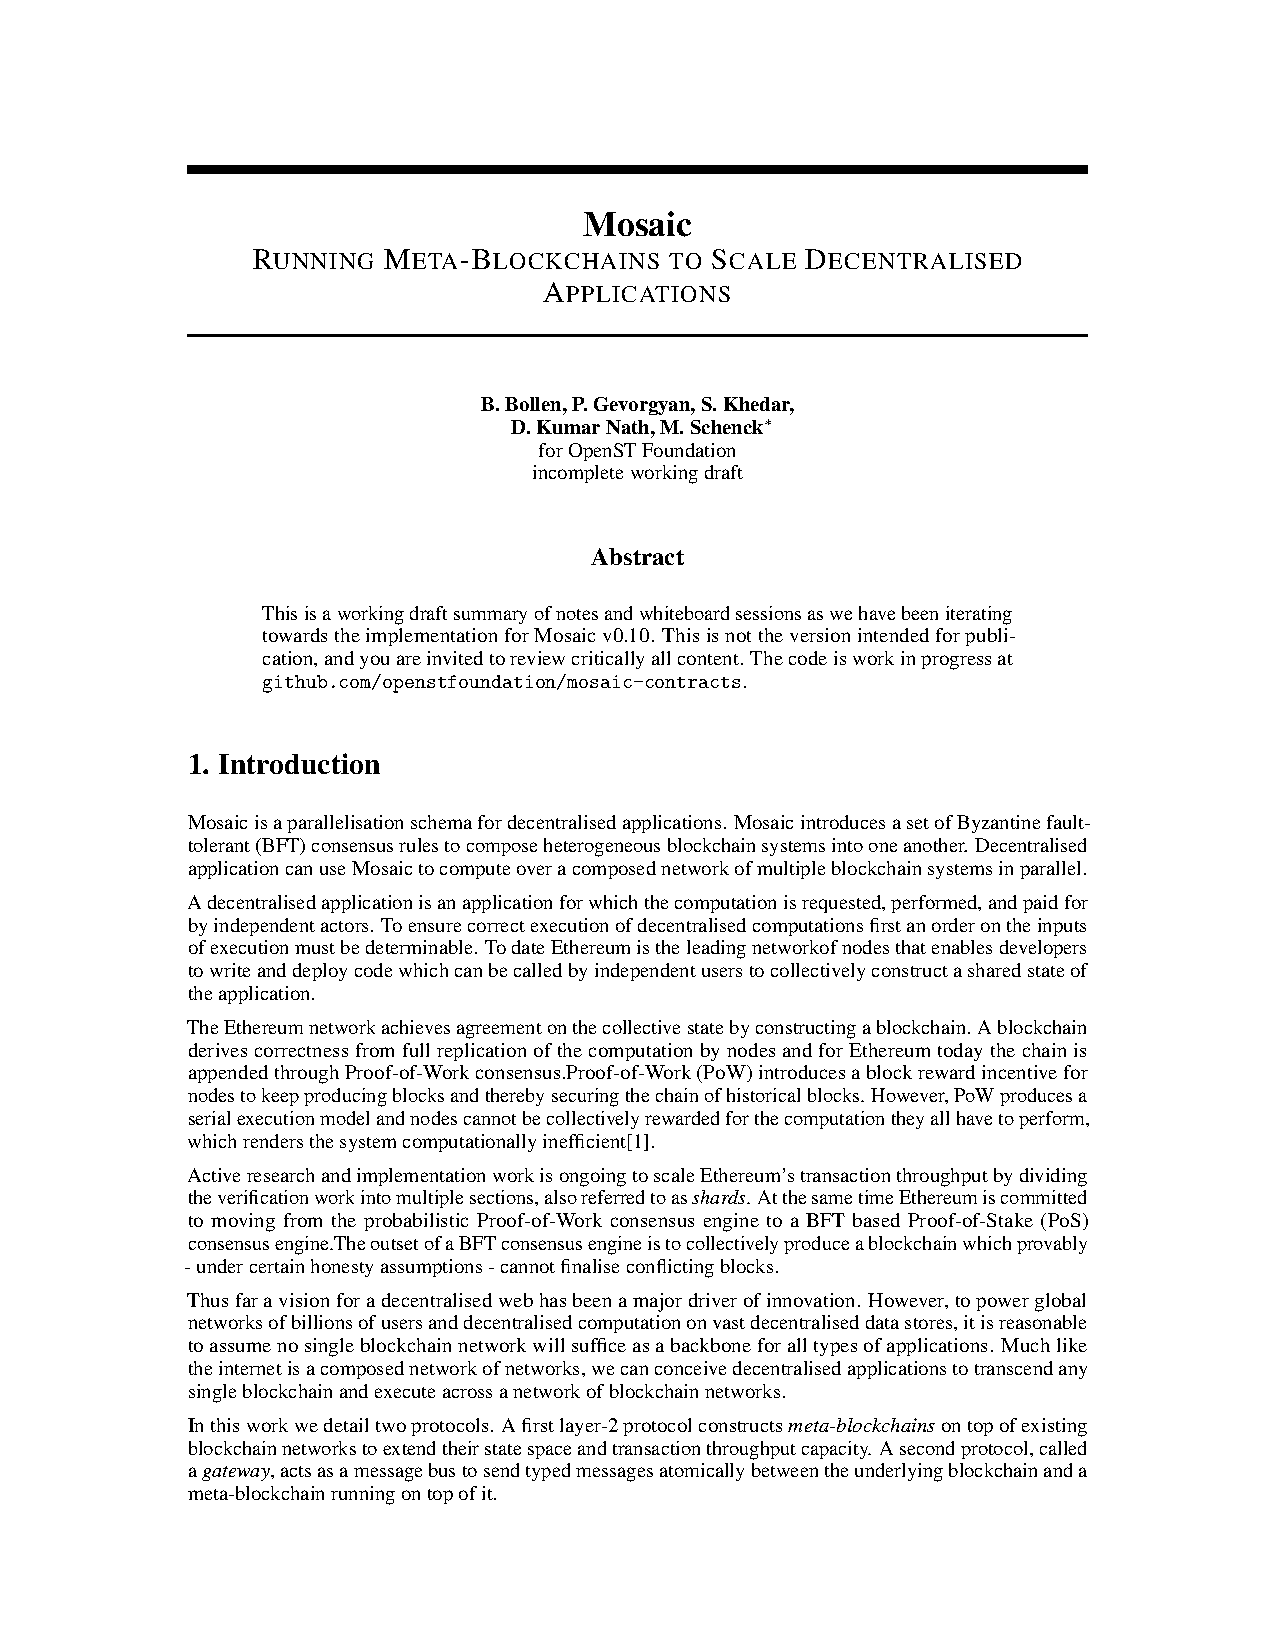
\includegraphics[width=\textwidth]{mosaic}
	\caption{\textbf{The Mosaic state transfer.}
		The closing of $\B_{\alpha-1}$ means that the finalised checkpoint $b_{A{}i}$ is the last block of $\B_{\alpha-1}$.
		Even though the details of $\B_\alpha$ will not be known until the opening is transferred to $A$,
		the first block in $\B_\alpha$ will be $b_{A{}i+1}$.
		Once a checkpoint is finalised after the OSTgas limit has been reached,
		% TODO V or a Mosaic node? where's the difference?
		$\V$ will signal the closing of $\B_\alpha$ to $O$.
	}
	\label{fig:mosaic}
\end{figure}

% TODO extend this paragraph
On the auxiliary chain, \emph{OSTgas} is the equivalent to gas on Ethereum.
For transactions to be included in blocks on auxiliary, a fee is paid for the consumed OSTgas.

% TODO possibly move this further up
Mosaic validators are allowed to commit every finalised state from auxiliary to origin.
However, that may be infeasible from an economic viewpoint of the validators.
Therefore, we propose points on the auxiliary chain where the validators must close the OSTblock.
Whenever a certain fixed limit of OSTgas has been spent on auxiliary since the opening of the OSTblock,
the validators \emph{must} close the OSTblock at the next finalised auxiliary checkpoint.
If a validator does not vote to commit that checkpoint,
its deposit can be slashed.
The OSTgas limit is marked in figure~\ref{fig:mosaic} by the dashed line.

Actors on the auxiliary chain have an economic incentive to finalise their state on origin.
The block creators of auxiliary will pay a fraction of their earned OSTgas to the Mosaic validators as a fee when the validators move the state to origin.
% TODO context and language
% TODO why?
Due to the OSTblocks, Mosaic validators can only copy the state from auxiliary to origin after the state of origin has been copied to auxiliary.
Thus, validators are incentivised to close an OSTblock and open a new one in order to earn the OSTgas fee for the transfer of auxiliary's state.

% TODO extend paragraph on punishment
It must be possible to hold Mosaic validators accountable if they misbehave.
In order to do so, anyone must be able to present proof of malicious actions on origin,
as the validators' deposits are stored there.
When a validator violates a slashing condition on auxiliary by making an illegal vote,
that fact is stored in the state of auxiliary.
Therefore, it can be proven against the state root of auxiliary.
Since the state root of auxiliary is available on origin,
the proof and the subsequent slashing can be carried out on origin as well.

% TODO extend paragraph on long range revisions
To prevent long range revisions, we apply the same rules that Casper applies:
after a Mosaic validator leaves the set of validators, its deposit is kept for another four months.
Casper votes on auxiliary can only be carried out up to three months into the past.
That leaves one month headroom to blame auxiliary's adversaries on origin and get its deposit slashed.
\end{comment}

\section{Gateway}

abstract:
the gateway protocol allows decentralized applications to deploy a message bus to send asynchronous messages between the state space of the origin blockchain and the state space of the auxiliary system supporting a specific meta-blockchain.
This allows tokens (ERC20, later non-fungible tokens) declared on the origin blockchain (Ethereum) to be locked and moved into the meta-blockchain where transactions can be finalised faster, and at a lower transaction cost. 

The gateway protocol is code-complete at github.com/openstfoundation/mosaic-contracts

%
% Section
%
\section{Outlook}

%
% Section
%
\section{Conclusion}

%\section{Appendix}




\bibliographystyle{naturemag}
\bibliography{mosaic.bib}

\end{document}
